\documentclass[11pt]{article}

%%% XeLaTeX Font Definitions

\usepackage{titlesec}
\usepackage{titling}
\usepackage{xunicode}
\usepackage{fontspec,xltxtra,xunicode}
\usepackage[table,xcdraw]{xcolor}
\defaultfontfeatures{Mapping=tex-text}

% Uncomment below to change default features 
%\setromanfont[Mapping=tex-text]{Hoefler Text}
%\setsansfont[Scale=MatchLowercase,Mapping=tex-text]{Gill Sans}
%\setmonofont[Scale=MatchLowercase]{Andale Mono}

% Specify different font for section headings
\newfontfamily\headingfont[]{Lucida Grande Bold}
\newfontfamily\titlefont[]{Optima}

\titleformat*{\section}{\Large\headingfont}
\titleformat*{\subsection}{\large\headingfont}
\titleformat*{\subsubsection}{\large\headingfont}
\renewcommand{\maketitlehooka}{\titlefont}

%%% Remove the "abstract" word before the abstract

\usepackage{abstract}
\renewcommand{\abstractname}{}    % clear the title
\renewcommand{\absnamepos}{empty} % originally center

%%% Actual Preamble

%\headheight=8pt
%\topmargin=3pt
%\textheight=624pt
%\textwidth=432pt
%\oddsidemargin=18pt
%\evensidemargin=18pt
\usepackage{amsmath}
\usepackage{amsfonts}
\usepackage{amssymb}
\usepackage{amsthm}
\usepackage{comment}
\usepackage{epsfig}
\usepackage{psfrag}
%\usepackage{sseq} (if you need to draw spectral sequences, please use this package, available at http://wwwmath.uni-muenster.de/u/tbauer/)
\usepackage{mathrsfs}
\usepackage{amscd}
\usepackage[all]{xy}
\usepackage{rotating}
\usepackage{lscape}
\usepackage{amsbsy}
\usepackage{verbatim}
\usepackage{moreverb}
\usepackage{mathdots}
\usepackage{setspace}
%\usepackage{eucal}
\usepackage{hyperref}
\usepackage{pgfplots}%http://www.ctan.org/pkg/pgfplots

\usepackage{listings}
\usepackage[margin=1in]{geometry}
\pagestyle{plain}
\theoremstyle{definition}
\newtheorem{theorem}{Theorem}%[section]
\newtheorem{prop}[theorem]{Proposition}
\newtheorem{lemma}[theorem]{Lemma}
\newtheorem{corollary}[theorem]{Corollary}
%\theoremstyle{definition}
\newtheorem{definition}[theorem]{Definition}
\newtheorem{notation}[theorem]{Notation}
\newtheorem{summary}[theorem]{Summary}
\newtheorem{note}[theorem]{Note}
\newtheorem{construction}[theorem]{Construction}
%\theoremstyle{remark}
\newtheorem{remark}[theorem]{Remark}
\newtheorem{example}[theorem]{Example}
\newtheorem{question}[theorem]{Question}
\DeclareMathOperator{\Aut}{Aut}
\DeclareMathOperator{\coeq}{coeq}
\DeclareMathOperator{\colim}{colim}
\DeclareMathOperator{\cone}{cone}
\DeclareMathOperator{\Der}{Der}
\DeclareMathOperator{\Ext}{Ext}
\DeclareMathOperator{\hocolim}{hocolim}
\DeclareMathOperator{\holim}{holim}
\DeclareMathOperator{\Hom}{Hom}
\DeclareMathOperator{\Iso}{Iso}
\DeclareMathOperator{\Map}{Map}
\DeclareMathOperator{\Tot}{Tot}
\DeclareMathOperator{\Tor}{Tor}
\DeclareMathOperator{\Spec}{Spec}
\newcommand{\TMF}{\mathit{TMF}}
\newcommand{\tmf}{\mathit{tmf}}
\newcommand{\Mell}{\mathcal M_{\mathit{ell}}}
\newcommand{\Mord}{\mathcal M_{\mathit{ell}}^{\mathit{ord}}}
\newcommand{\Mss}{\mathcal M_{\mathit{ell}}^{\mathit{ss}}}
\newcommand{\Mbar}{\overline{\mathcal M}_{\mathit{ell}}}
\newcommand{\Mfg}{\mathcal M_{\mathit{FGL}}}
\newcommand{\MU}{\mathit{MU}}
\newcommand{\MP}{\mathit{MP}}
\newcommand{\Lk}{L_{K(n)}}
\newcommand{\Lone}{L_{K(1)}}
\newcommand{\Ltwo}{L_{K(2)}}
\newcommand{\Sp}{\mathbf{Sp}}
\newcommand{\Eoo}{E_\infty}
\newcommand{\Aoo}{A_\infty}
\newcommand{\CP}{\mathbb{CP}^\infty}
\newcommand{\GL}{\mathit{GL}}
\newcommand{\gl}{\mathit{gl}}
\newcommand{\nn}{\nonumber}
\newcommand{\nid}{\noindent}
\newcommand{\ra}{\rightarrow}
\newcommand{\la}{\leftarrow}
\newcommand{\xra}{\xrightarrow}
\newcommand{\xla}{\xleftarrow}
\newcommand{\weq}{\xrightarrow{\sim}}
\newcommand{\cofib}{\rightarrowtail}
\newcommand{\fib}{\twoheadrightarrow}
 \newcommand{\xhdr}[1]{\vspace{2mm}\noindent{{\bf #1.}}}

\def\llarrow{   \hspace{.05cm}\mbox{\,\put(0,-2){$\leftarrow$}\put(0,2){$\leftarrow$}\hspace{.45cm}}}
\def\rrarrow{   \hspace{.05cm}\mbox{\,\put(0,-2){$\rightarrow$}\put(0,2){$\rightarrow$}\hspace{.45cm}}}
\def\lllarrow{  \hspace{.05cm}\mbox{\,\put(0,-3){$\leftarrow$}\put(0,1){$\leftarrow$}\put(0,5){$\leftarrow$}\hspace{.45cm}}}
\def\rrrarrow{  \hspace{.05cm}\mbox{\,\put(0,-3){$\rightarrow$}\put(0,1){$\rightarrow$}\put(0,5){$\rightarrow$}\hspace{.45cm}}}
\def\cA{\mathcal A}\def\cB{\mathcal B}\def\cc{\mathbf C}\def\cd{\mathbf D}
\def\ce{\mathcal E}\def\cf{\mathcal F}\def\cG{\mathcal G}\def\cH{\mathcal H}
\def\cI{\mathcal I}\def\cJ{\mathcal J}\def\cK{\mathcal K}\def\cL{\mathcal L}
\def\cM{\mathbf M}\def\cN{\mathcal N}\def\cO{\mathbf O}\def\cP{\mathcal P}
\def\cQ{\mathcal Q}\def\cR{\mathcal R}\def\cS{\mathcal S}\def\cT{\mathcal T}
\def\cU{\mathcal U}\def\cV{\mathcal V}\def\cW{\mathcal W}\def\cX{\mathcal X}
\def\cY{\mathcal Y}\def\cZ{\mathcal Z}
\def\AA{\mathbb A}\def\BB{\mathbb B}\def\CC{\mathbb C}\def\DD{\mathbb D}
\def\EE{\mathbb E}\def\FF{\mathbb F}\def\GG{\mathbb G}\def\HH{\mathbb H}
\def\II{\mathbb I}\def\JJ{\mathbb J}\def\KK{\mathbb K}\def\LL{\mathbb L}
\def\MM{\mathbb M}\def\NN{\mathbb N}\def\OO{\mathbb O}\def\PP{\mathbb P}
\def\QQ{\mathbb Q}\def\RR{\mathbb R}\def\SS{\mathbb S}\def\TT{\mathbb T}
\def\UU{\mathbb U}\def\VV{\mathbb V}\def\WW{\mathbb W}\def\XX{\mathbb X}
\def\YY{\mathbb Y}\def\ZZ{\mathbb Z}

\newcommand{\MFGL}{\mathcal M_{\mathit{FGL}}}
\newcommand{\calO}{{\mathcal O}}
\newcommand{\calC}{{\mathcal C}}
\newcommand{\set}{{\mathrm{Set}}}
\newcommand{\Deltab}{{\mathbf \Delta}}
\newcommand{\spet}{\mathrm{Spec}^\mathrm{\acute{e}t}}
\newcommand{\Z}{\mathbb Z}
\DeclareMathOperator{\Spf}{Spf}

\usepackage{fancyhdr}
\setlength{\headheight}{15.2pt}
\pagestyle{fancy}

\lhead{2016-17}
\chead{Information Theory}
\rhead{Manan Shah}

\begin{document}
\title{\headingfont{Information Theory}}
\author{Manan Shah\\ \texttt{manan.shah.777@gmail.com} \\ The Harker School}
\maketitle
\begin{abstract}
This document contains lecture notes from Harker's Advanced Topics in Mathematics class in Information Theory, Parts I and II. These notes were taken using TeXShop and \LaTeX2$\epsilon$ and will be updated for each class. The reader is advised to note any errata at the source control repository \texttt{https://github.com/mananshah99/infotheory}.
\end{abstract}
\tableofcontents
\newpage

%% Notes start here

\section{August 22, 2016}
\subsection{Class Overview}
\begin{figure}[h]
\centering
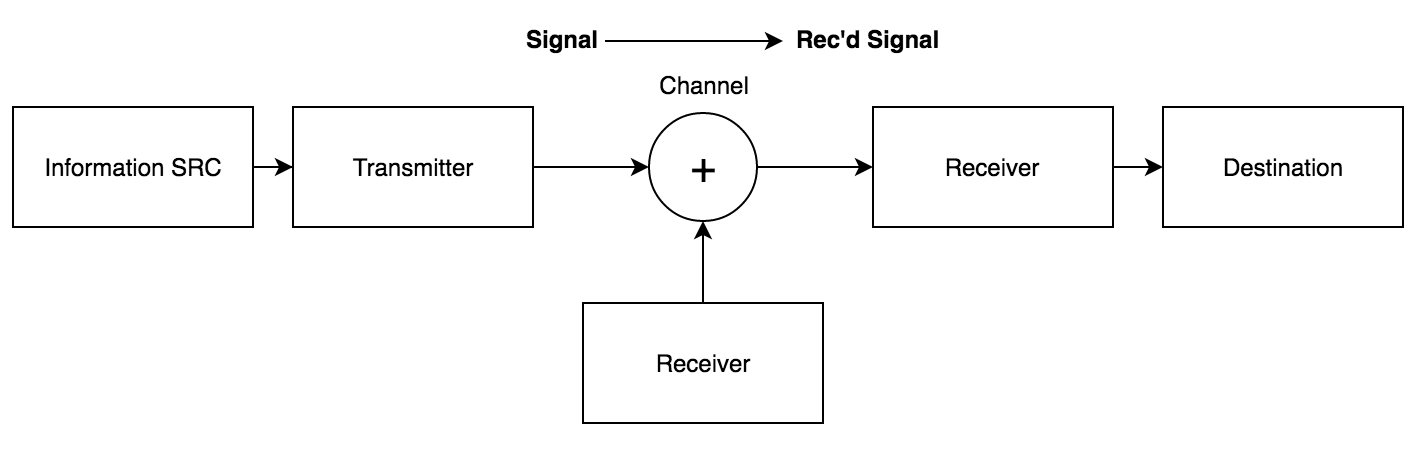
\includegraphics[scale=0.5]{pipeline}
\end{figure}
Information may be conveyed in multiple ways; for example, by a person talking, a video, or pictures. Our goal is to model this kind of information as a system with one output and no input. The information is therefore a box that emits output probabilistically, and we will therefore be spending 1-2 weeks on probability, specifically regarding distribution functions and expectation. This is illustrated in the ``information source'' box---the job of the information source is to \textbf{provide the signal}. 

We will next define the compression problem; having obtained numbers as a stream, the problem is to remove the redundancy in a stream. In particular, we will discuss both lossless and lossy compression. One of the most critical ideas in this course is that of entropy, and we will define the concept (in general, a notion of how much information is originating from the source). We will also discuss the sensibility of such a definition and potentially expand upon it. An overarching concept here will be our definition of the performance of a compression algorithm via the source compression theorem and the boundedness of compression algorithms. This is illustrated in the ``transmitter'' box---the job of the transmitter is to \textbf{remove all redundancy}.

We will subsequently discuss the channel circle, which we will model with conditional probability distribution functions (PDFs). The output of this box, the receiver signal, is input to the receiver box, which has the job of \textbf{reconstruction of the signal and the noise}; this is known as the coding problem. Much like the compression problem of the source, the channel has the capacity problem (how much information can be transmitted?). And similar to the compression theorem, we will discuss the channel coding theorem, which will help us determine which parts of a code will require more redundancy for transmission. 

We will finally discuss Shannon's theorem, in which he states that a communication with no loss and arbitrary cost (due to a constraint on the amount of bandwith, power, etc.) is possible if the entropy of the source $H$ is less than the capacity of the channel $C$. In our course, we will first discuss the pipeline for lossless compression and then move to lossy compression.

\section{August 24, 2016}
Knowing what a random variable is and what it means is important for the source to transmitter relationship. 
\subsection{Random Variables}
\definition A random variable is a real-valued function of the outcome of an experiment. By definition, it is not deterministic.
\notation We will represent random variables with capital letters (for example, $X, Y, Z$).
\example[What are Random Variables?] (a) A coin is tossed ten times. Determine the number of heads obtained from the coin toss. The number of heads is the random variable in this case. (b) Given two rolls of die, identify their sum (a random variable) and the second roll raised to the fifth power (another random variable). (c) The time to transmit a message, the delay with which a message is received, and the number of errors in a message are both themselves random variables. \\

\noindent Two types of random variables exist; discrete variables and continuous variables. 
\definition[Discrete RV] A discrete random variable is one that has a finite set of outcomes (or is countably infinite), and has a probability associated with each outcome. 
\definition[Continuous RV] A continuous random variable is one that has a non-finite, uncountable set of outcomes. 

\example Define the function 
\begin{equation*}
sgn(a) = \begin{cases}
1 &a > 0\\
0 & a = 0 \\
-1 & a < 0
\end{cases}
\end{equation*}
The variable $a$ is a continuous random variable, while $sgn(a)$ is a discrete function (with outputs $\in \{1, 0, -1\}$)
\subsubsection{Probability Mass Function (pmf)}
Probability mass functions are functions of a discrete random variable, describing all instances of a random variable occurring and its associated probabilities. Define $X$ as a random variable, and write $P(X = x)$ as $p_X(x)$. Then $\sum_x p_X(x) = 1$. Consider two tosses of a coin, letting $X$ equal the number of heads obtained. We therefore have 
\begin{equation*}
p_X(x) = \begin{cases}
1/4 & x =0\\
1/2 & x=1\\
1/4 & x=2 \\
\end{cases}
\end{equation*}
note that $p_X(x)$ is clearly a discrete function that takes on values $x \in \{0, 1, 2 \}$ with respective output probabilities. 
\subsubsection{Probability Density Function (pdf)}
%\begin{figure*}[h]
%\centering
%    \begin{tikzpicture}
%    \path[draw](0,0)--(0,5);
%    \path[draw](0,0)--(5,0);
%     \path[draw] (0,0) -- (2,2) -- (4,0);
%    \end{tikzpicture}
%\end{figure*}
Probability density functions are functions of a continuous random variable. Define $X$ as a random variable. In this case, the expression $P(X = x)$ is meaningless (in fact, it is defined as 0). The probability of a range of values from $x = a$ to $x = b$ is more relevant; in particular, $\int_{-\infty}^{\infty}p_X(x) = 1$. 

\example Edgar's driving time to school is between 15 and 20 minutes if it is sunny and between 20 and 25 minutes if it is a rainy day. Assume a day is sunny with $2/3$ probability and rainy with $1/3$ probability. Construct the respective PDF. \\

\noindent The PDF construction is quite simple; remember that $\int_{-\infty}^{\infty}p_X(x) = 1$. 
\begin{equation*}
p_X(x) = \begin{cases}
2/15 & 15 \leq x \leq 20\\
1/15 & 20 \leq x \leq 25 \\
0 & x \geq 25 \\
\end{cases}
\end{equation*}

\subsubsection{Types of Random Variables}
We will define these distributions in terms of a coin toss. 

\xhdr{Bernoulli (Discrete)} Toss a coin, and it define the probability of heads as $p$. The respective PMF is 
\begin{equation*}
p_X(x) = \begin{cases}
p & x = 1\\
(1-p) & x = 0
\end{cases}
\end{equation*}

\xhdr{Binomial (Discrete)} Toss a coin $N$ times, and define $x$ as the number of heads obtained in $N$ tosses. Let $N = 10$, and define the probability of heads as $p$. Then the respective PMF is 
\begin{equation*}
p_X(x) = \begin{cases}
(1-p)^{10} & x = 0\\
{10 \choose 2}p^2(1-p)^8 & x = 2 \\
\dots & $other values of $ x \in [0, 10] \cap \mathbb{N}
\end{cases}
\end{equation*}

\xhdr{Geometric (Discrete)}  Repeatedly toss a coin until the first ``success.'' This means that we may theoretically have countably infinite $P(X = 1), P(X = 2), P(X = 3), \dots$ output values. Define success to be a head, and the probability of heads as $p$. Then, we have
\begin{equation*}
p_X(x) = \begin{cases}
p & x = 1\\
(1-p)p & x = 2 \\ 
(1-p)^2p & x = 3 \\
\dots & $other values of $ x
\end{cases}
\end{equation*}

\xhdr{Poisson (Discrete, $\sim$ Binomial)} Instead of tossing a biased coin and counting the number of heads (a binomial distribution), count the number of times one must replace a biased lightbulb in a time $t$ (with the lightbulb being on or off). This makes the poisson distribution a discrete one. Our distribution function is 
\begin{equation*}
p_X(x) = \frac{e^{-\lambda} \lambda^x}{x!}
\end{equation*}
where $\lambda$ is an arbitrary constant. The number of decay events in some radioactive element, for example, may be modeled using a Poisson distribution. Anything that involves units of time and something happening within a period of time $t$ may include a Poisson distribution. 

\xhdr{Exponential (Continuous, $\sim$ Geometric)} Given a biased lightbulb, identify the amount of time until the bulb burns out. Examples of the use of this function include rates (as opposed to numbers defined with the Poisson distribution). The PDF is defined as
\begin{equation*}
p_X(x) = \begin{cases}
\lambda e^{-\lambda x} & x \geq 0 \\
0 & $otherwise$
\end{cases}
\end{equation*}
where $\lambda$ is an arbitrary constant.

\xhdr{Gaussian (Continuous)} If one does enough experiments of a binomial random variable, the distribution will end up looking like a Gaussian. The PDF is
\begin{equation*}
p_X(x) = \frac{1}{\sqrt{2\pi\sigma^2}}e^{\frac{-(x - \mu)^2}{2\sigma^2}}
\end{equation*}
where $\mu$ and $\sigma$ are parameters that can be treated as constants. 
\section{August 26, 2016}
\subsection{Properties of Random Variables}
We will be defining expectation and variance, and deriving equations regarding these properties of random variables. 
\subsubsection{Expectation (Mean) of a Random Variable}

\xhdr{Discrete} The notation is $E[X]$, where $X$ is the random variable. We have $$E[X] = \mu = \sum_x x_i p(x_i)$$For example, the expected value of rolling a die is 3.5. 

\xhdr{Continuous} The notation is again $E[X]$, where $X$ is the random variable. We have $$E[X] = \mu = \int_{-\infty}^\infty x p(x) dx$$

\noindent In fact, it is possible to find the expected value of any function of a random variable. For example, $$E[X^2] = \sum_x x_i^2 p(x_i)$$ $E[X]$ is called the ``first moment'' of a variable, and $E[X^2]$ is called the ``second moment.''

\subsubsection{Variance of a Random Variable}

We will denote the variance of a random variable as $V[X]$ (in class, this is denoted $Var[X]$). The variance depends on the expectation, and is written as $$V[X] = E[(X - E[X])^2] = E[X^2] - E[X]^2$$It is possible to expand this condensed form in both discrete and continuous forms. 

\xhdr{Discrete} $V[X] = \sum_x(x_i - \mu)^2p(x_i)$
\xhdr{Continuous} $V[X] = \int_{-\infty}^\infty (x_i - \mu)^2 p(x_i)dx$

\noindent The variance is always a positive quantity, and the standard deviation $\sigma = \sqrt{V[X]}$.

\subsubsection{The Mean and Variance of a Bernoulli Distribution}
Recall the definition of a Bernoulli random variable,
\begin{equation*}
p_X(x) = \begin{cases}
p & x = 1\\
(1-p) & x = 0
\end{cases}
\end{equation*}
We can write 
\begin{align*}
E[X] &= \sum_x x_i p(x_i) \\
&= 1(p) + 0(1-p) \\
&= p
\end{align*} 
The variance is defined as $E[(x-\mu)^2]$, so we have
\begin{align*}
V[X] &= \sum_x (x_i - p)^2 p(x_i) \\
&= (1-p)^2 p + (0-p)^2 (1-p) \\
&= p(1-p)
\end{align*}

\subsubsection{The Mean and Variance of a Geometric Distribution}
Recall the definition of a geometric random variable,
\begin{equation*}
p_X(x) = \begin{cases}
p & x = 1\\
(1-p)p & x = 2 \\ 
(1-p)^2p & x = 3 \\
\dots & $other values of $ x
\end{cases}
\end{equation*}
We can write %(todo: clean the tex up)
\begin{align*}
E[X] &= p(1-p)^0 + 2p(1-p)^1 + \dots \\
&= p(1-p)^0 + p(1-p)^1 + p(1-p)^2 + \dots = 1 \\
&\qquad \qquad \: \: \: \: \: \: + p(1-p)^1 + p(1-p)^2 + \dots = 1-p \\
& \qquad \qquad \qquad \qquad \qquad \: \: + p(1-p)^2 + \dots = (1-p)^2
\end{align*}
The critical insight here is that $2p(1-p)$ can be written as $p(1-p) + p(1-p)$, and $3p(1-p)^2$ can be written the same way, with each sub-series forming a geometric series. We then sum the resulting geometric series $1 + (1-p) + (1-p)^2 + \dots$, yielding $E[X] = \frac{1}{p}$. \\

\noindent The variance is defined as $V[X] = E[X^2] - E[X]^2$, which simplifies (after much algebra) to $$V[X] = \frac{1-p}{p^2}$$

\subsubsection{The Mean and Variance of a Binomial Distribution}
Recall the definition of a binomial random variable,
\begin{equation*}
p_X(x) = \begin{cases}
(1-p)^{10} & x = 0\\
{10 \choose 2}p^2(1-p)^8 & x = 2 \\
\dots & $other values of $ x \in [0, 10] \cap \mathbb{N}
\end{cases}
\end{equation*}
We can write
\begin{align*}
E[X] &= \sum_x x_i p(x_i) \\
&= 0p(0) + 1p(1) + 2p(2) + \dots \\
&= 1\left(p(1-p)^{n-1} {n \choose 1}\right) + 2 \left(p^2(1-p)^{n-2} {n \choose 2} \right) + \dots \\
&=  np \left({n-1 \choose 0} (1-p)^{n-1} + {n-1 \choose 1} p(1-p)^{n-2} + {n-1 \choose n-1}p^{n-1}\right) \\
&= np((p+1)-p)^{n-1} \\
&= np
\end{align*}

\noindent Note that a binomial random variable is really just a bunch of independent binomial random variables added up. So we can sum the variances to obtain $V[X] = np(1-p)$. In retrospect, we could have done the same for $E[X]$.

\section{August 30, 2016}

\subsection{Wrapping up Means and Variances} 

Recall the following facts from last time. Bernoulli: $E[X] = p$, $V[X] = p(1-p)$. Binomial: $E[X] = np$, $V[X] = np(1-p)$. Geometric: $E[X] = 1/p$, $V[X] = (1-p)/p^2$. 

\subsubsection{The Mean and Variance of a Poisson Distribution}
We may go over this in the future. For now, note that $E[X] = V[X] = \lambda$. 

\subsubsection{The Mean and Variance of a Exponential Distribution}
Here, we have $E[X] = 1/\lambda$ and $V[X] = 1/\lambda^2$. The derivation for $E[X]$ is as follows, noting that $p(x) = \lambda e^{-\lambda x}$. So,
\begin{align*}
E[X] &= \int_{0}^{+\infty} x \lambda e^{-\lambda x} dx \\
	&= \lambda \left[ \frac{-x}{\lambda} e^{-\lambda x} \bigg|_0^\infty+ \frac{1}{\lambda} \int_0^{+\infty}e^{-\lambda x}dx \right] \\
	&= 0 + \left(\frac{-1}{\lambda} \right)e^{-\lambda x}\bigg|_0^\infty \\
	&= \frac{1}{\lambda}
\end{align*}

\subsubsection{The Mean and Variance of a Gaussian Distribution}
Remember that the PDF is
\begin{equation*}
p_X(x) = \frac{1}{\sqrt{2\pi\sigma^2}}e^{\frac{-(x - \mu)^2}{2\sigma^2}}
\end{equation*}
where $\mu$ and $\sigma$ are parameters that can be treated as constants. The integration involves the error function, and yields $E[X] = \mu$ and $V[X] = \sigma^2$. 

\subsection{Linearity of Expectation}
The central idea is that, if one has properties of random variables $X$ and $Y$, it would be nice to also know properties about the sum $X + Y$. 

\theorem[Linearity of Expectation] $E[X + Y] = E[X] + E[Y]$.
\begin{proof}
This statement is the same as $$\sum_x \sum_y (x + y)p(X = x, Y = y)$$where the probability function is certainly not conditional, but may not be represented as the product of both individual probabilities as no assumptions are made of independence. This may be rewritten as $$\sum_x \sum_y x p(X = x, Y = y) + \sum_x \sum_y y p(X = x, Y = y)$$which is equivalent to $$\sum_x x \sum_y p(X =x, Y = y) + \sum_y \sum_x y p(X =x, Y = y)$$Note that, in the left sum indexed by $y$, the probabilities of $y$ sum to 1 so the resulting value is simply $p(X = x)$. The same is true for the right sum, yielding $$\sum_x xp(X =x) + \sum_y y p(Y = y)$$which completes the proof. 
\end{proof}
\noindent Note that this result is not true for the variances; i.e.  $V[X+Y] = V[X] + V[Y]$. The linearity of variances is only true when $X$ and $Y$ are independent (really, uncorrelated). 

\example{Let $Y = aX + b$}. We have $E[Y] = aE[X] + b$. The linear shift does not affect variance, and so our resulting variance is $V[Y] = a^2V[X]$. 

\example{You have an urn with three types of balls: 8 blue, 4 white, and 2 orange. Choose two balls at random. You win two dollars for every blue ball, lose one dollar for every white ball, and are not changed by an orange ball. Determine all values of $X$, your winnings, the probability of $X$, and $E[X]$.} \\

\noindent A listing of possible winnings is as follows: 4, 2, 1, 0, -1, -2. $P(4) = \binom{8}{2}/\binom{14}{2}$. $P(2) = \binom{8}{1} \binom{2}{1} / \binom{14}{2}$. $P(1) = \binom{8}{1} \binom{4}{1} / \binom{14}{2}$. $P(0) = \binom{2}{2} / \binom{14}{2}$. $P(-1) = \binom{2}{1} \binom{4}{1} / \binom{14}{2}$. $P(-2) = \binom{4}{2} / \binom{14}{2}$. Multiply each value with its probability to obtain $E[X] = 12/7 \approx 1.71$.

\example One of the numbers $(1-10)$ is randomly chosen. You are to try to guess the number by asking yes or no questions. Compute the expected number of questions if (a) your ith question is ``is it $i$?'', and (b) with each question, you try to eliminate $1/2$ of the remaining as nearly as possible. \\

\noindent (a) The expected value is $$E[X] = \frac{1}{10} \cdot 1 + \frac{1}{10} \cdot 2 + \frac{1}{10} \cdot 3 + \cdots = 5.5$$ 

\noindent (b) Draw a decision tree (for example, first split has left branch $1,2,3,4,5$ and left branch has $6,7,8,9,10$). Count the probability for each number of moves and obtain $$E[X] = 4 \cdot \frac{4}{10} + 3 \cdot \frac{6}{10} = 3.4$$

\example Suppose that the average numbers of cars abandoned in a week on a certain highway is 2.2. Approximate the probability that there will be (a) no abandoned cars this week and (b) at least two abandoned cars in the next week. \\

\noindent (a) Use a Poisson distribution. $E[X] = \lambda = e^{-2.2}$. \\

\noindent (b) This is expressed as $1 - p_X(x = 1) - p_X(x = 0)$ which equals $1 - 2.2e^{-2.2} - e^{-2.2}$. 

\section{September 1, 2016}
This class was primarily reviewing Problemset 2. 
\theorem[Bayes] $P(A|B) \cdot P(B) = P(A \& B) = P(A \cap B) = P(B|A) \cdot P(A)$.

\section{September 6, 2016}
We will first go over some problems, and then talk more about information sources and whether it makes sense to model them as random variables. 
\subsection{Review Problems}
\example$X$ is a random variable with probability with probability distribution function. Let 
\begin{equation*}
f(x) = \begin{cases}
c(1-x^2) & -1 < x < 1\\
0 & x = $anything else$ \\
\end{cases}
\end{equation*}
(a) What is $c$? $\int f(x) dx = 1$, so we have $(cx - \frac{cx^3}{3}|_{-1}^1 = 1$, and $c = 3/4$. \\
(b) Recall the definition of $E[X] = \int xf(x) dx$. So, we have $E[X] = \int_{-1}^1 x (3/4) (1-x^2)dx = 0$. 

\example The PDF of lifetime of a certain type of electronic device is
\begin{equation*}
f(x) = \begin{cases}
10/x^2&  x > 10 \\
0 & x \leq 10 \\
\end{cases}
\end{equation*}
(a) What is $P(X > 20)$? Integrate from 20 to infinity and solve to obtain $1/2$. \\
(b) What is the probability that, of 6 such types of devices, at least three will function at least 15 hours? State assumptions. Assume that each case is independent. We have $P(X > 15) = 2/3$. So our expression for exactly 3 is $$1 - P(0) - P(1) - P(2)$$which equals $$1 - \binom{6}{0}(1/3)^6 - \binom{6}{1}(1/3)^5 (2/3) - \binom{6}{2} (1/3)^4 (2/3)^2$$

\example Find $E[X]$ of the following \\
(a) \begin{equation*}
f(x) = \begin{cases}
5/x^2&  x > 5 \\
0 & x \leq 5 \\
\end{cases}
\end{equation*}
(b) \begin{equation*}
f(x) = \begin{cases}
(x/4)e^{-x/2}&  x > 0 \\
0 & $otherwise$ \\
\end{cases}
\end{equation*}
(a) is 0, (b) is 4 (integrate by parts twice)

\subsection{Information Sources}

Can these sources be modeled as a system with no input and one output and output emits symbols probabilistically?

\begin{table}[h]
\centering
\label{my-label}
\begin{tabular}{|l|l|l|l|l|}
\hline
\rowcolor[HTML]{EFEFEF} 
Type      & \begin{tabular}[c]{@{}l@{}}Source\\ (Black Box)\end{tabular} & Data                                                       & Characteristics of PDF                                                                   & Can you send less?                                                    \\ \hline
e-mail    & computer                                                     & text                                                       & frequency of letters, greetings, formatting                                              & Possible                                                              \\ \hline
telephone & receiver                                                     & sound                                                      & \begin{tabular}[c]{@{}l@{}}decibel range, tone, background noise, \\ pauses\end{tabular} & \begin{tabular}[c]{@{}l@{}}Possible\\ (similar to email)\end{tabular} \\ \hline
images    & camera                                                       & pixels                                                     & \begin{tabular}[c]{@{}l@{}}background, same pixel values for large\\ areas\end{tabular}  & Possible                                                              \\ \hline
video     & camera                                                       & \begin{tabular}[c]{@{}l@{}}series of\\ images\end{tabular} & stationary objects in video                                                              & Possible                                                              \\ \hline
\end{tabular}
\end{table}

\section{September 8, 2016}
\subsection{Modeling English Probabilistically}
Today, we will go through the same thought experiment that Claude Shannon performed. Looking at English text, Shannon first analyzed whether it could be modeled probabilistically. \\

\xhdr{Zeroth Order} A simplistic zeroth order approximation involves assuming uniform distribution across all letters. This may be conducted by rolling a 27 sided die. A sample output might look like: \\
XFOML RXKHRJFFJUJ ZLPWCFWKCYJ FFJEYVKCDSGHYD QPAAMKBZAACCIBZLHJQD\\
\xhdr{First Order} A first order approximation leverages the probabilities of certain letters. For example, $P_{X}(E) \approx 0.13$ and $P_{X}W \approx 0.02$. A sample output might look like: \\
OCRO HLI RGWR NMIELWIS EU LL NBNESBEYA THEEI \\
\xhdr{Second Order} A second order approximation utilizes the probability of a letter appearing given the preceding letter. A sample output might look like: \\
ON IE ANTSOUTINYS ARE T INCTORE ST BE S DEAMY ACAIW D ILONONASIVE\\
\xhdr{nth Order} We can extend this out to an $n$th order approximation, which uses information about the preceding $n-1$ letters to predict the value of the $n$th character. The larger the value of $n$, the more like English the model's output becomes. 

\subsection{Shannon's Assumptions about Sources}
Shannon assumed that all sources are {\bf ergodic}. Ergodic sources are those whose distributions do not change with time. While this may not hold true universally, it is a reasonable approximation for most practical applications of his work. 

\end{document}
